\documentclass[12pt]{article}
\usepackage[margin=1in]{geometry} 
\usepackage{amsmath,amsthm,amssymb,amsfonts,algpseudocode,graphicx,mathtools}

\newcommand{\N}{\mathbb{N}}
\newcommand{\Z}{\mathbb{Z}}

\newenvironment{problem}[2][Problem]{\begin{trivlist}
\item[\hskip \labelsep {\bfseries #1}\hskip \labelsep {\bfseries #2.}]}{\end{trivlist}}
%If you want to title your bold things something different just make another thing exactly like this but replace ``problem'' with the name of the thing you want, like theorem or lemma or whatever

\newtheorem{theorem}{Theorem}
\newtheorem{lem}{Lemma}
\DeclarePairedDelimiter{\ceil}{\lceil}{\rceil}

\begin{document}
%\renewcommand{\qedsymbol}{\filledbox}
%Good resources for looking up how to do stuff:
%Binary operators: http://www.access2science.com/latex/Binary.html
%General help: http://en.wikibooks.org/wiki/LaTeX/Mathematics
%Or just google stuff

\title{CMPSCI-683 Homework Assignment \#2: Constraint Satisfaction and Adversarial Search}
\author{Patrick Pegus II}
\maketitle

\begin{problem}{1}
	Show that any CSP that has a finite domain for each variable can be transformed into a CSP with only binary constraints. Follow these steps:
	\begin{enumerate}
		\item Show how a single ternary constraint such as $A+B=C$ can be turned into three binary constraints by using an auxiliary variable.
			(Hint: consider a new variable $AB$ whose domain is pairs of numbers.)
		\item Next, show how constraints with more than three variables can be treated similarly.
		\item Finally, show how unary constraints can be eliminated by altering the domains of variables.
	\end{enumerate}
	\begin{enumerate}
		\item Let $D_{AB}=\{a+b|a \in D_a, b \in D_b\}$ be the domain of the variable $AB$.
			Then $A+B=C$  can be replaced by $AB=C$, $A = a$, $B = b$.
		\item Iteratively remove variables from non-binary constraints, such as
			\begin{align*}
				V_1 * \dots * V_i * V_{i+1} * \dots * V_m = V_n
			\end{align*}
			by replacing it with
			\begin{align*}
				V_1 * \dots * V_iV_{i+1} * \dots *V_m = V_n \text{, } V_i = v_i \text{, } V_{i+1} = v_{i+1}
			\end{align*}
			until only binary constraints exist.
			Where $D_{V_iV_{i+1}} = \{v_i * v_{i+1}| v_i \in D_{v_i}, v_{i+1} \in D_{v_{i+1}}\}$.
		\item Any unary constraint $U$ that imposes a condition on variable $V$, such as $U(V)=True$,
			can be eliminated after reducing the domain of $V$ to only values $v$ where $U(v)=True$.
	\end{enumerate}
\end{problem}
\begin{problem}{2}
	Sudoku is a fairly old puzzle that is now a worldwide phenomenon.
	You can type ``sudoku'' into Google, or read the Wikipedia article to get more information than you could possibly imagine.
	Key facts about standard Sudoku puzzles:
	\begin{itemize}
		\item Every puzzle has a unique solution.
		\item Every puzzle is solvable without trial-and-error, given suitable inference methods.
		\item The designated difficulty of a puzzle is usually determined by the difficulty of the inference methods required to solve it.
	\end{itemize}
	In addition to the rules, many web sites offer extensive discussion of methods that humans can use to solve Sudoku without using trial-and-error search.
	You need to write a program that can solve Sudoku problem instances. To test your program, you should apply it to the following 16 puzzles:
	See \texttt{/data/sudoku\_puzzles/}. \\
	These puzzles are from ``Sudoku: Easy to Hard'', by Will Shortz.
	The original collection includes 100 puzzles (from 1-25 are 'light and easy', 26-50 are 'moderate', 51-75 are 'demanding', and 76-100 are 'beware! very challenging').
	Each puzzle is stored in a file that looks as follows: \\

	\begin{tabular}{ccccccccc}
		- & 1 & 9 & - & - & - & - & - & - \\
		- & - & 8 & - & - & 3 & - & 5 & - \\
		- & 7 & - & 6 & - & - & - & 8 & - \\
		- & - & 1 & - & - & 6 & 8 & - & 9 \\
		8 & - & - & - & 4 & - & - & - & 7 \\
		9 & 4 & - & - & - & - & - & 1 & - \\
		- & - & - & - & - & 2 & - & - & - \\
		- & - & - & - & 8 & - & 5 & 6 & 1 \\
		- & - & 3 & 7 & - & - & - & 9 & - \\
	\end{tabular}
	\begin{enumerate}
		\item Explain how Sudoku can be represented as a CSP (how many variables are needed? what are their domains? what are the constraints?). 

			Sudoku can be represented as a CSP with a matrix of variables $M=V_{ij}$ for the entries in the puzzle.
			$i$ and $j$ are the row and column index, respectively.
			Since $i$ and $j$ are integers in $[1,9]$, there are 81 variables.
			The domains of each $V_{ij}$ are the integers in $[1,9]$.
			The constraints are:
			\begin{enumerate}
				\item $V_{ij} \neq V_{ik}$, if $j \neq k$
				\item $V_{ij} \neq V_{kj}$, if $i \neq k$
				\item When $M$ is partitioned into 9 3x3 matrices $m = V_{ab}$, $V_{ab} \neq V_{cd}$ , if $a \neq c$ or $b \neq d$.
			\end{enumerate}
		\item Write a program that can read a Sudoku puzzle from a file and solve it using the backtracking-search algorithm that was discussed in class (slide 16).
			Keep in mind that instead of representing the constraints explicitly in your program, it might be easier to write a function that checks if a given variable assignment results in a conflict with the values already placed in its row/column/square.
			Try to solve a few of the Sudoku instances using this algorithm and make sure that it works.
			Explain why can plain backtracking search solve Sudoku puzzles quickly despite the size of the problem?

			Please see the \texttt{simpleBacktrackSearch} function in csp.py for the implementation of the backtracking algorithm.
			Plain backtracking search can solve easier Sudoku puzzles quickly because constraints of the puzzle often render variable assignments inconsistent quickly.
			Suppose no variable assignment could be determined to be inconsistent until all variables were assigned, then plain backtracing would have to enumerate all
			possible combinations of variable values in the worst case.
		\item Now instrument backtracking-search so that it counts the total number of guesses made.
			Whenever the backtracking algorithm prepares to loop through a list of $k>0$ possible values, we will say that $k-1$ guesses are made.
			(This way, the algorithm is still charged for guessing even if it is lucky and its first value choice succeeds.)
			Show the numbers of guesses made for each of the 16 instances in the above collection.
			Try both plain backtracking and backtacking with the MRV (minimum remaining values) heuristic.

			\begin{tabular}{c|ccc}
				& \multicolumn{2}{c}{Guess count} & \\
				Puzzle & Plain  & MRV \\
				\hline
				1 & 130 & 171 \\
				2 & 832 & 200 \\
				10 & 11567 & 1268 \\
				15 & 43417 & 3198 \\
				25 & \textbf{367431} & 33045 \\
				26 & \textbf{497103} & 38149 \\
				48 & \textbf{176487} & 99282 \\
				51 & \textbf{514666} & 26076 \\
				62 & \textbf{423581} & 1319 \\
				76 & \textbf{367354} & 126492 \\
				81 & \textbf{300203} & 72855 \\
				82 & \textbf{393530} & \textbf{428756} \\
				90 & \textbf{457224} & 320336 \\
				95 & \textbf{431714} & \textbf{619242} \\
				99 & \textbf{343688} & 30412 \\
				100 & \textbf{378558} & 78429 \\
			\end{tabular} \\
			As shown the MRV heuristic drastically reduced guessing, allowing most of sudoku puzzles to be completed without inference within the 5 minute timeout.
			Guess counts occurring during a timeout are bold face.
			One iteration of AC-3 was run on the puzzle domain so that MRV makes a difference.
		\item Please see the inferences method of the Sudoku class in sudoku2.py for the implementation of the waterfall.
			Please see the ac3 method of the Sudoku class in sudoku2.py for the implementation of AC-3.

			\begin{tabular}{c|ccc}
				& \multicolumn{2}{c}{Guess count} & \\
				Puzzle & AC-3 & AC-3 + Neighbors Can't \\
				\hline
				1 & 0 & 0 \\
				2 & 0 & 0 \\
				10 & 0 & 0 \\
				15 & 0 & 0 \\
				25 & 0 & 0 \\
				26 & 2 & 2 \\
				48 & 19 & \textbf{18} \\
				51 & 7 & 7 \\
				62 & 4 & 4 \\
				76 & 10 & 10 \\
				81 & 4 & 4 \\
				82 & 35 & 35 \\
				90 & 44 & \textbf{42} \\
				95 & 20 & \textbf{19} \\
				99 & 12 & 12 \\
				100 & 10 & 10 \\
			\end{tabular} \\
			The Neighbors Can't inference method assigns a value to a variable if the variable's neighbors assignments or domain do not include that value.
			Arc consistency limits the domain of a variable assigning a value to a variable if the domain size becomes 1.
			The Neighbors Can't method assigns a value to a variable if no other neighbor could possibly take on that value.
			As shown in the table above it made little improvement.
			It would have been more effective had it checked neighbors in a row, then column, then submatrix, instead of all neighbors at once.
			Please see the neighborsCant method of the Sudoku class in sudoku2.py for the implementation of this method.
		\item Propose a method to determine the difficulty of a given Sudoku puzzle automatically using your solver. You don't have to implement your technique.

			The difficulty of a puzzle can be estimated by the number of iterations through each inference method.
	\end{enumerate}
\end{problem}
\begin{problem}{3}
	Consider the following game tree in which the static heuristic scores are given for all the tip nodes.
	\begin{figure}[h]
		\centering
		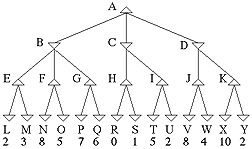
\includegraphics[width=0.5\textwidth]{fig/gametree.jpg}
		%\caption{Nodes expanded and compute time as a function of the number of cities to be toured during 50 A$^*$ searches. The number of cities is a uniform random number between 1 and 15.}
		\label{fig:gametreee}
	\end{figure}
	\begin{enumerate}
		\item What move should MAX choose?

			MAX should move to node D.
		\item What nodes would not need to be examined using the alpha-beta algorithm -- assuming that nodes are examined in left-to-right order?

			Nodes O, Q, I, T, U, and Y would not need to be examined.
	\end{enumerate}
\end{problem}
\begin{problem}{4}
	Suppose we play a variant of Tic-Tac-Toe in which each player sees only his or her own moves.
	If the player makes a move on a square occupied by an opponent, the board ``beeps'' and the player gets another try.
	Would the backgammon model (the EXPECTIMAX-EXPECTIMIN algorithm described in Section 5.5) suffice for this game, or would we need something more sophisticated? Why?

	\vspace{0.25cm}
	Something more sophisticated is needed.
	This variant of Tic-Tac-Toe is partially observable.
	Therefore, a deterministic terminal test and utility function would not suffice.
	It would also be difficult to use chance nodes to create a probability distribution over available actions,
	since the probability of available actions are not only influenced by the number of moves so far, but also the strategy of the opponent.
\end{problem}
\begin{problem}{5}
	Consider the following procedure for choosing moves in games with chance nodes:
	\begin{itemize}
		\item Generate a suitable (say, 1000) dice-roll sequences down to a suitable depth (say, 8).
		\item With known dice rolls, the game tree becomes deterministic. For each dice-roll sequence, solve the resulting deterministic game tree using alpha-beta.
		\item Use the results to estimate the value of each move and choose the best one.
	\end{itemize}
	Will this procedure work well? Why (not)?

	\vspace{0.25cm}
%	This procedure will not work well because the actiaction $b$ reons that should be undertaken as a result of more probable dice rolls will dominate the estimate.
%	This may result in poor decision making should an improbable dice roll actually happen.
%	Consider this simplified example of an unfair coin where the probability of heads is 0.9, if the coin flip results in heads then actions $a$ and $b$ result in rewards of 1 and -1, respectively.
%	However, if the coin flip is heads, $a$ and $b$ result in -1 and 1, respectively.
%	The result of the procedure will be to choose $a$h
	This procedure will work well. 
	The large number of sequences causes the action returned most often by alpha-beta over the sequences to converge to the action resulting in the state with highest expected utility, as Expectiminimax does.
	When compared to Expectiminimax, it reduces time complexity by $\frac{1000}{d^8}$ where $d$ is the number of distinct dice rolls.
	Additionally, the probability of each dice roll can be unknown.
\end{problem}

\end{document}
